\documentclass[12pt]{article}
\usepackage[top=1in, bottom=1in, left=1in, right=1in]{geometry}

\usepackage{setspace}
\onehalfspacing

\usepackage{amssymb}
%% The amsthm package provides extended theorem environments
\usepackage{amsthm}
\usepackage{epsfig}
\usepackage{times}
\renewcommand{\ttdefault}{cmtt}
\usepackage{amsmath}
\usepackage{graphicx} % for graphics files

% Draw figures yourself
\usepackage{tikz} 

% writing elements
\usepackage{mhchem}

% The float package HAS to load before hyperref
\usepackage{float} % for psuedocode formatting
\usepackage{xspace}

% from Denovo Methods Manual
\usepackage{mathrsfs}
\usepackage[mathcal]{euscript}
\usepackage{color}
\usepackage{array}

\usepackage[pdftex]{hyperref}
\usepackage[parfill]{parskip}

% math syntax
\newcommand{\nth}{n\ensuremath{^{\text{th}}} }
\newcommand{\ve}[1]{\ensuremath{\mathbf{#1}}}
\newcommand{\Macro}{\ensuremath{\Sigma}}
\newcommand{\rvec}{\ensuremath{\vec{r}}}
\newcommand{\omvec}{\ensuremath{\hat{\Omega}}}
\newcommand{\vOmega}{\ensuremath{\hat{\Omega}}}
%---------------------------------------------------------------------------
%---------------------------------------------------------------------------
\begin{document}
\begin{center}
{\bf NE 155/255, Fall 2019 \\
Nuclear Physics Basics and Terms\\
September 9, 2019}
\end{center}

\setlength{\unitlength}{1in}
\begin{picture}(6,.1) 
\put(0,0) {\line(1,0){6.25}}         
\end{picture}

A primary goal of nuclear reactor analysis and design is the reliable 
prediction of neutron population production and loss rates. In order to fully
describe neutron transport through media, we need to describe neutron motion 
and neutron interactions with matter.

To begin determining probabilities of neutron-nuclear reactions, we will first 
review the aspects of nuclear physics that are relevant for fission chain 
reactions. 

\subsection*{Nuclear Physics of Chain Reactions}

Notation reminder: \ce{^{A}_{Z}X} indicates that chemical element $X$ has $Z$ 
protons (atomic number) and $A$ total nucleons (protons + neutrons; mass 
number). This leaves $N$ neutrons.

Excited states are written as \ce{^{A}_{Z}X^*}, and metastable/isomeric as
\ce{^{A}_{Z}X^m}.

There are two types of \textbf{basic nuclear transformations}:

\begin{enumerate}
\item spontaneous disintegration: The spontaneous decay of unstable nuclei, 
      with emission of particles or radiation

\[X \rightarrow Y + y + Q\]

These are probabilistic events that depend only on the type of nucleus.

\item induced by collision: An event in which, because of interaction with a 
      particle or radiation (a projectile), a nucleus (target) is changed in 
      mass, charge or energy state, and particles or radiation is emitted.

\[x + X \rightarrow Y + y + Q\]
\end{enumerate}

Here, $y$ and $x$ are typically $\alpha$, $\beta$, or $\gamma$ and $Q$ is
energy.

\underline{Examples} of common reactions:
\begin{itemize}
\item Potential elastic scattering $(n,n)$: \ce{^1_0 n} + \ce{^A_Z X}
      $\rightarrow$ \ce{^1_0 n} + \ce{^A_Z X}
\item Resonance elastic scattering $(n,n)$: \ce{^1_0 n} + \ce{^A_Z X}
      $\rightarrow$ (\ce{^A_Z X$^*$}) $\rightarrow$ \ce{^1_0 n} + \ce{^A_Z X}
\item Inelastic scattering $(n,n')$: \ce{^1_0 n} + \ce{^A_Z X} $\rightarrow$
      (\ce{^A_Z X$^*$}) $\rightarrow$ \ce{^1_0 n} + \ce{^A_Z X} + $\gamma$
\item Radiative capture (absorption) $(n,\gamma)$: \ce{^1_0 n} + \ce{^A_Z X}
      $\rightarrow$ (\ce{^A_Z X$^*$}) $\rightarrow$ \ce{^{A+1}_Z X} + $\gamma$
\item Fission (absorption) $(n,f)$: \ce{^1_0 n} + \ce{^A_Z X} $\rightarrow$
      \ce{^{A1}_{Z1} X} + \ce{^{A2}_{Z2} X} + (a few)\ce{^1_0 n}
\item Charged-Particle Reactions (absorption): $(n,\alpha)$ \ce{^1_0 n} +
      \ce{^A_Z X} $\rightarrow$ \ce{^{A-3}_{Z-2} Y} + \ce{^{4}_{2} He}; \\
      \hspace*{17 em}$(n,p)$  \ce{^1_0 n} + \ce{^A_Z X} $\rightarrow$
      \ce{^{A}_{Z-1} Y} + \ce{^1_1 p}
\item Neutron-Producing Reactions (absorption): $(n,2n)$\ce{^1_0 n} +
      \ce{^A_Z X} $\rightarrow$ \ce{^{A-1}_{Z} X} + 2\ce{^1_0 n}
\end{itemize}

Which reaction happens depends on the type of nucleus, the energy of the 
incoming neutron, and statistics. We can, fortunately, draw general categories 
for many types of reactions:

\begin{figure}[h!]
    \begin{center}
    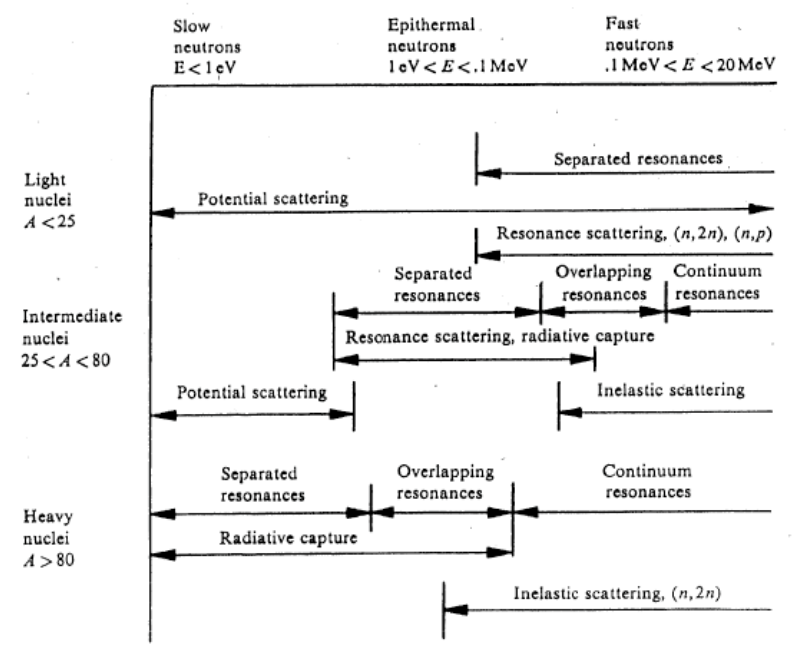
\includegraphics[keepaspectratio, width = 5 in]{reactionenergy}
    \caption{Neutron Interactions by Energy and Atomic Number}
    \label{fig:reactions}
    \end{center}
\end{figure}

Nuclear reactions have to obey a set of \textbf{Conservation Laws}, which 
govern what actually happens in the transformations. 

\begin{itemize}
\item Conservation of mass/energy: The total energy of the system before 
      nuclear transformation must be equal to the total energy of the system 
      after the transformation.
\item Conservation of Linear Momentum: Total linear momentum of the system (a  
      vector) before nuclear transformation must be equal to the total linear 
      momentum of the system (a vector) after the transformation.
\item Conservation of charge: Total charge of the system before nuclear
      transformation must be equal to the total charge of the system after the 
      transformation.
\item Conservation of nucleons: Total number of nucleons (protons and 
      neutrons) of the system before nuclear transformation must be equal to 
      the total number of nucleons (protons and neutrons) of the system after 
      the transformation.
\end{itemize}

The conservation laws govern what reactions can happen. What reactions 
actually happen govern the neutron population in a reactor. 

What we'll cover next are the definitions and terms we will use to describe 
neutrons in six-dimensional phase space: $(x,y,z,\vOmega, E)$.

\subsection*{Definitions}

\begin{figure}[h!]
    \begin{center}
    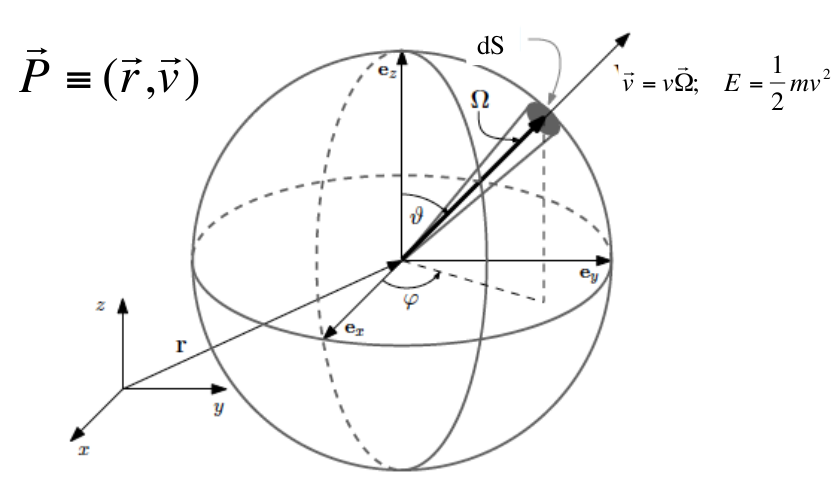
\includegraphics[keepaspectratio, width = 4 in]{phase-space}
    \end{center}
    \caption{Schematic of Phase Space}
    \label{fig:phase_space}
\end{figure}

Spatial logistics
\begin{itemize}
\item $d\vec{r} = d^3r$ = ordinary volume =
      $r^2 \sin(\theta) d\theta d\varphi dr$
\item $v$ = speed (scalar)
\item $\vec{v}$ = $v\vOmega$ = velocity (vector)
\item $d\vec{v} = d^3v$ = velocity volume =
      $v^2 \sin(\theta)d\theta d\varphi dr$
\item $v = \sqrt{(2E)/m}$ where $m$ is the rest mass of the particle. Thus, we 
      can relate energy and speed.

\item $\vOmega$: unit directional vector in velocity space,
      $\vec{v} = v\vOmega$
\item $d\vOmega = \sin(\theta)d\theta d\varphi =  d^2\Omega$
%\item thus $d\vec{v} = v^2 dv d\vOmega$
\end{itemize}

These are the possible reactions we're generally going to worry about:

\hspace*{1em}total (t): all interactions. We can break total into:
\begin{itemize}
\item scattering (s): a neutron interacts with an atom and bounces off either 
      elastically or inelastically.
\item absorption (a): a neutron is absorbed by a nucleus.
\item fission (f): cause the nucleus to split into two pieces, releasing more 
      neutrons.
\end{itemize}

Physics terms we will use:

\begin{enumerate}
\item \textbf{microscopic x-sec} ($\sigma$, [$cm^2$]): measure of the 
      probability that an incident neutron will collide with a specific 
      nucleus; $\sigma_j$ indicates a specific reaction, e.g.\ $j=f$ is 
      fission.
\item \textbf{macroscopic x-sec} ($\Sigma$ [$cm^{-1}$]): measure of the 
      probability per unit path length that an incident neutron will collide 
      with a target \[\Sigma_j = \sigma_j N\:,\] where N is the atomic density 
      of the target. The total cross section is simply the sum of all possible 
      reaction types, $j$. 

If a material is made of multiple isotopes, the material macroscopic cross 
section is also the sum over all materials, $i$:

\[
\Sigma_i(\vec{r}, E, t) =
\sum_{j=1}^J  N_j(\vec{r}, t)\sigma_{i,j}(E)
\qquad
\Sigma_t(\vec{r}, E, t) =
\sum_{j=1}^J \sum_{i=1}^I N_j(\vec{r}, t)\sigma_{i,j}(E)
\]

\end{enumerate}

\end{document}